\chapter{Structure d'un système asservi}
\section{Notion d'automatique}

L'automatisme regroupe plusieurs disciplines telles que la \textbf{modélisation}, \textbf{l'analyse} et la \textbf{commande des systèmes dynamiques}.
Un système est dit automatique si il peut réaliser un certain nombre d'opération sans l'aide de l'Homme. \newline

Deux grands types de systèmes automatiques :

\begin{itemize}
    \item La logique combinatoire et séquentielle
    \item Les systèmes asservis
\end{itemize}

\newpage
\section{Notion de système}

Un système est un ensemble de composants fonctionnant entre eux pour réaliser un certain nombre de tâches.
\begin{itemize}
    \item  Systèmes \textbf{continus}
    \item  Systèmes \textbf{linéaires}
    \item  Système \textbf{invariants}
    \item Systèmes \textbf{monovariables}
    \item Systèmes \textbf{multivariables}
\end{itemize}

Continu : un système est dit continu si, pour une entrée $e$ et une sortie $s$, les fonctions $e$ et $s$ sont continues sur tout leurs intervalle de définition. \newline

Linéaire : un système est dit linéaire si il respecte la propriété suivante : soit $I$ et $J$ les ensembles de définition de $e$ et $s$, respectivement entrée et sortie du système, on a, $\forall t,u \in I, \forall \lambda,\mu \in R, e(\lambda t + \mu u) = \lambda e(t) + \mu e(u)$, de même pour la fonction s.
Exmple de non-linéarités : hystérésis, saturation, balours mécaniques, thermiques et électriques\newline

Invariant : le système ne change pas au cours du temps. Par exemple, pas usure dûs aux frottements, pas de fatigue mécanique \newline

Monovariable : une entrée, une sortie \newline

Multivariable : plusieurs entrées, plusieurs sorties \newpage 

\section{Modélisation d'un système :}
\large{
Représentation des \textbf{SLCI} (pour une sortie y, entrée u):
}
\subsection{En continu : }

Equation différentielle du système :
\begin{center}
\Large{\fbox{{$\sum_{i=0}^{n_d} \alpha_{i} y^{(i)}(t)$} = {$\sum_{j=0}^{n_n} \beta_{j} u^{(j)}(t)$}}}
\end{center}
Transformée de Laplace de l'équation différentielle du système : 
\begin{center}
\Large{{$\sum_{i=0}^{n_d} \alpha_{i} Y^{i}(p)$} = {$\sum_{j=0}^{n_n} \beta_{j} U^{j}(p)$}}
\end{center}
Réponse impulsionnelle :
\begin{center}
\Large{\fbox{$y(t)=h(t)*u(t) = $\(\int_{}^{} h(\tau)u(\tau - t) \,d\tau\)}}     
\end{center}
Fonction de transfert :
\begin{center}
    \Large{\fbox{$Y(p) = H(p)U(p)$ avec : $H(p) = $\(\int_{}^{} h(t)e^{-pt} \,dt\)}}
\end{center}
Représentation d'état : 
\[
\left \{
\begin{array}{c @{=} c}
    \dot x(t) & Ax(t) + Bu(t)\\
    y(t) & Cx(t) + Du(t)
\end{array}
\right.
\]
\subsection{En Discret :}
Equation aux différences :
\begin{center}
\Large{\fbox{$\sum_{i=0}^{n_d} \alpha_{i} y[k-i]$ = {$\sum_{j=0}^{n_n} \beta_{j} u[k-j]$}}}
\end{center}
Réponse impulsionnelle :
\begin{center}
\Large{\fbox{$y[k]=h[k]*u[k] = \sum_{i=0} h[k]u[k - i]$}}   
\end{center}
Représentation d'état : 
\[
\left \{
\begin{array}{c @{=} c}
    \dot x[k] & Ax[k] + Bu[k]\\
    y[k] & Fx[k] + Gu[k]
\end{array}
\right.
\]
\newpage
\section{Type de commande :}
\begin{itemize}
    \item Commande passive : modification du système en lui-même.
    \item Commande en boucle ouverte (BO) : modification de l'entrée en fonction de la sortie
    \item Commande en boucle fermée (BF) : recalcul de l'entrée en fonction de la valeur mesurée en sortie
\end{itemize}
\section{Structure d'un système asservi monovariable}
\begin{center}
    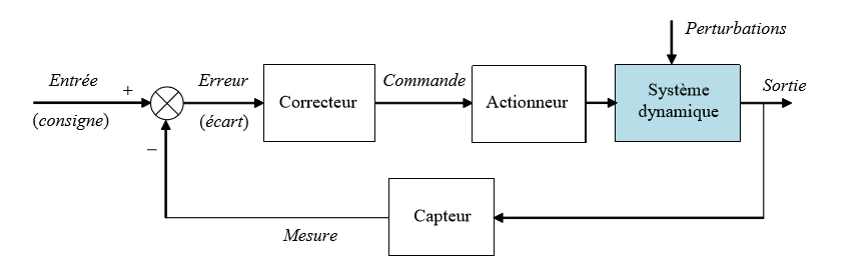
\includegraphics[scale=0.8]{Pics/FTBF.png}
    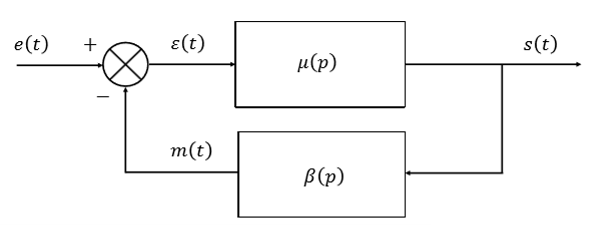
\includegraphics[scale=0.8]{Pics/assev2ndOrdre.png}
\end{center}

Pour un système du second ordre, la fonction de transfert en forme canonique s'écris de la manière suivante : 
\begin{center}
    \Large{\fbox{$H(p)=\frac{S(p)}{E(p)}=
    \frac{K}{1+
    2\xi \frac{p}{\omega_{0}} +
    \frac{p^{2}}{\omega_{0}^{2} }}$}} 
\end{center}
\newpage
Avec :
\large{
    \[
\left \{
\begin{array}{c @{=} c}
    \omega_{0} & \sqrt{\frac{K}{\tau}}\\
    \xi & \frac{1}{2\sqrt{K\tau}}
\end{array}
\right.
\]
}
\newline


\begin{center}
\begin{itemize}
    \item
    \Large{$
    \omega_{c} = 
    \frac{1}{\tau}
    \sqrt{\frac{
    -1 + \sqrt{1+4K^{2}\tau^{2}}
    }
    {2}
    }
    $} 

    \item \Large{$
\Delta \phi =  
\frac{\pi}{2}- \frac{360}{2\pi}\arctan{(\omega_{c}\tau) =
\frac{\pi}{2}- \frac{360}{2\pi}\arctan{(\frac{1}{\tau}
    \sqrt{\frac{
    -1 + \sqrt{1+4K^{2}\tau^{2}}
    }
    {2}
    }\tau)}}
$}

    \item \Large{$t_{m}=\frac{\pi}{\omega_{0}\sqrt{1-\xi^{2}}}$}

    \item \Large{$\omega_{a}=\omega_{0}\sqrt{1-\xi^{2}}$}
    \end{itemize}
\end{center}

\newpage
\section{Critère des systèmes asservis}
\subsection{Rapidité}
Temps de réponse à 5\% $t_{r5\%}$ : c'est la valeur temporelle à partir de laquelle la valeur de la sortie prise en $t=t_m$ est comprise entre 95\% et 105\% de la valeur finale $v_f$.
\begin{center}
    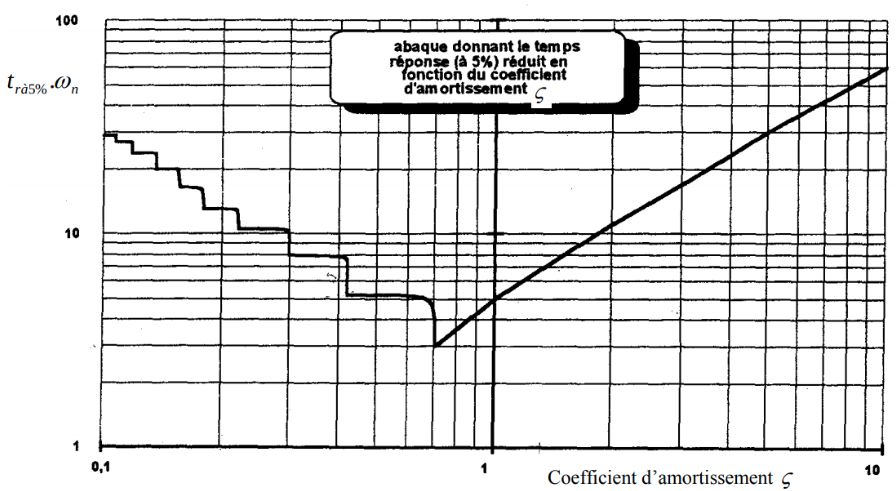
\includegraphics[scale=0.7]{Pics/rapidite_abaque.png}
\end{center}
\newpage
\subsection{Stabilité}
Critère de stabilité : \textbf{nombre de dépassements, marge de phase, propriétés sur les pôles.} \newline

\begin{itemize}
    \item un système est dit \textbf{stable} si ses pôles \footnote{Les pôles sont les racines du polynôme au dénominateur de la fonction de transfert sous forme canonique} sont à partie réelle strictement négative. C'est-à-dire que : \newline
Pour une fonction de transfert \newline \large{$H(p)=\frac{S(p)}{E(p)}=\frac{\sum_{i=0}^{n_d} \alpha_{i} p^{i}}
{\sum_{j=0}^{n_n} \beta_{j} p^(j)}$} le système est dit stable si \newline

\Large{$\forall \lambda \in \mathbf{C}$, $\lambda$ racine de $\sum_{j=0}^{n_n} \beta_{j} p^{j}, Re(\lambda) < 0$}
    \item Plus $M\phi \nearrow$, plus la stabilité $\nearrow$ avec \fbox{$tan(\phi) = \frac{Im(H(j\omega))}{Re(H(j\omega))}$}
\end{itemize}
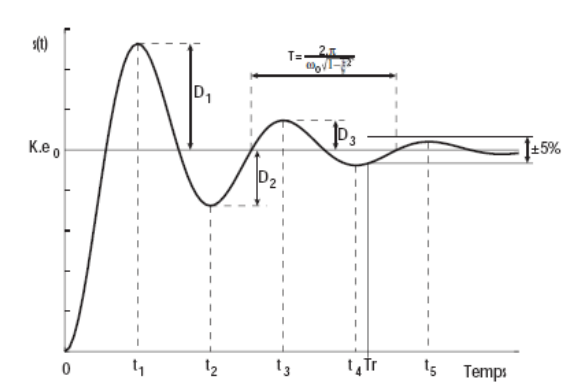
\includegraphics[scale=0.87]{Pics/stab.png} \newline
Temps entre deux pseudo-périodes :     \fbox{\Large{$t_{m}=\frac{\pi}{\omega_{0}\sqrt{1-\xi^{2}}}$}} \newline
Pseudo pulsation :     \fbox{\Large{$\omega_{a}=\omega_{0}\sqrt{1-\xi^{2}}$}}
\newpage
Temps de la k-ième pseudo-période : 
Amplitude du k-ième dépassement (avec $E_{0}$ l'amplitude de l'entrée):
\begin{center}
    \fbox{\Large{$D_{k}=kE_{0}e^{-k\frac{\pi\xi}{\sqrt{1-\xi^{2}}}}$}}
\end{center}
\subsection{Précision}
Critère de précision : la valeur finale doit se rapprocher le plus possible de la valeur de consigne. On considère alors un système précis si l'erreur statique \footnote{L'erreur statique est la valeur de l'erreur quand le régime est permanent. $\epsilon_{s}$ ne dépend pas de $t$ par conséquent} $\epsilon_s = 0$. \newline

Théorème de la valeur finale : \newline
\begin{center}
    \fbox{$\lim_{t \to \infty} s(t) = lim_{p \to 0} pS(p) = v_{f}$}    
\end{center}
Théorème de la valeur initiale : \newline
\begin{center}
    \fbox{$\lim_{t \to 0} s(t) = lim_{p \to \infty} pS(p) = v_{i}$}
\end{center}

\newpage
\section{Formule de Black}
\begin{center}
    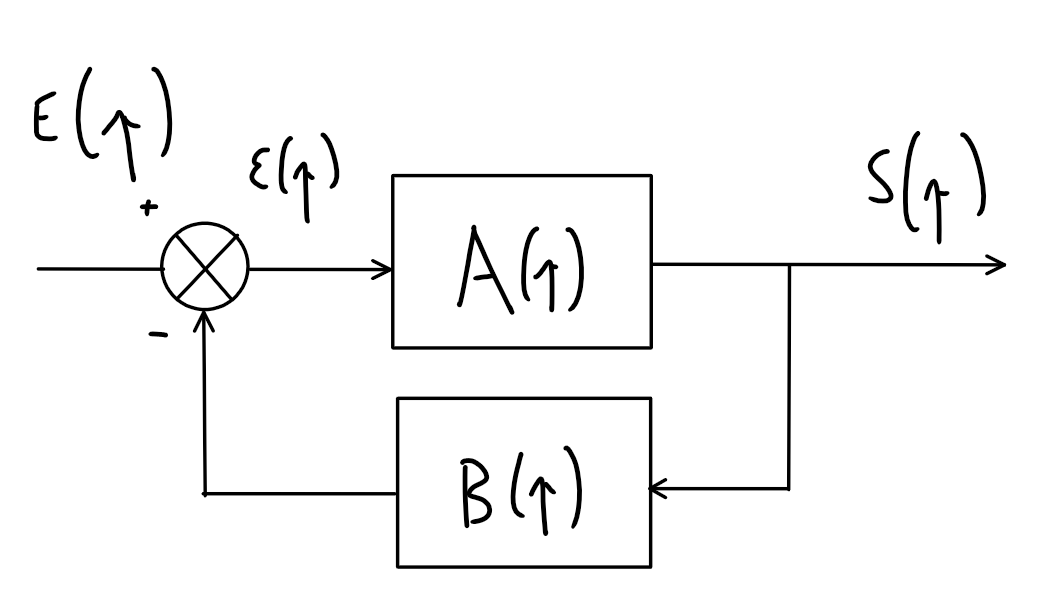
\includegraphics[scale=0.3]{Pics/Black.png}
\end{center}

On a :
\Large{$\epsilon (p) = E(p) - BS(p)$} \newline
\Large{$S(p) = A\epsilon (p)$} \newline
Donc :
\Large{$\frac{S(p)}{A} = E(p) - BS(p) \Longleftrightarrow S(p) = \frac{AE(p)}{1+AB}$}
\begin{center}
\LARGE{\fbox{$H(p) = \frac{S(p)}{E(p)} = \frac{A(p)}{1 + A(p)B(p)}$}}   
\end{center}

\section{Correcteurs}
Différents types de correcteur :
\begin{itemize}
    \item Proportionnel
    \item Dérivé
    \item Intégral
\end{itemize}
On peut proposer un correcteur qui est une composition des correcteurs usuels :
\begin{itemize}
    \item Proportionnel Intégral (PI)
    \item Dérivé Intégral (DI)
    \item Proportionnel Intégral Dérivé (PID)
\end{itemize}
\newpage
\subsection{Proportionnel}
\subsection{Intégral}
\subsection{Dérivé}
\section{Diagramme de Bode}
\newpage
\section{Diagramme de Nyquist}
Pour étudier les critères d'un système asservi, on peut aussi utiliser le diagramme de Nyquist \newline 

Diagramme ($(Im(H(j\omega)),Re(H(j\omega)))$.  

\begin{center}
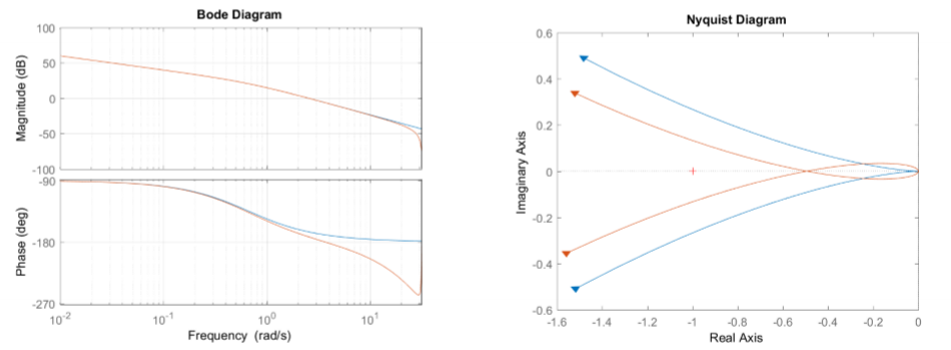
\includegraphics[scale=0.7]{Pics/Nyquist.png}    
\end{center}
\newpage
\section{Transformée en $z$}
\subsection{Principe de fonctionnement}
\begin{center}
    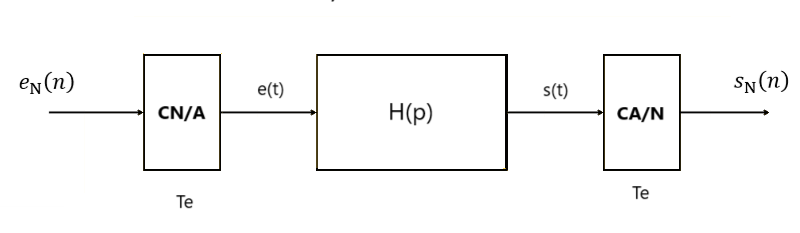
\includegraphics[scale=0.8]{Pics/TransformeeZ.png}
\end{center}
\subsection{Propriétés}
\begin{center}
    \Large{\fbox{$Z(x(t)) = x_{N}(z)$}} \newline
    
    \Large{\fbox{$Z(\frac{dx(t)}{dt}) = z^{-1}x_{N}(z)$}} \newline

    \Large{\fbox{$
    H_{N}(z) = 
    \frac{S_{N}(z)}{E_{N}(z)} = 
    (1 - z^{-1})Z(\frac{H(p)}{p})
    $}} \newline  
\end{center}
